\chapter{Introduction}%
\label{ch:introduction}

This thesis presents the development and simulation-based validation of control strategies for fingertip positioning and force control for a \mbox{6-DOF} tendon-driven hand exoskeleton. The exoskeleton is developed by the N-Squared lab at Friedrich-Alexander Universität Erlangen-Nürnberg (FAU), Erlangen, Germany, and is intended for use in spinal-cord-injured (SCI) patients, with the goal of improving hand function and independence. 

\section{Motivation}
SCI-patients may end up having the ability to control their muscles, reduced or even lost due to their nerves being damaged. They may retain their limbs, but are unable to control them at will. This differs from people that are born with missing limbs, or that through life lose their limbs. In these cases, total reconstruction of the limbs, like with prosthetics are needed to restore movement. Instead of prosthetics, people with muscular dysfunction will need something to move their still existing limbs for them. This is usually done by an orthosis, also refered to as an exoskeleton. 

Research has shown that some SCI-patients with muscular dysfunction, still retain some motor neuron activity in their forearm \parencite{tingWearableNeuralInterface2019}. This activity can be measured with intramuscular electromyography (iEMG) \parencite{ICSGlossary}, and classifiers or regression models can then be used on this data to interpret the user's intent. With the intent of the user, an external exoskeleton could then be used to move the fingers in accordance to what the user intended, regaining the users independence and improving their quality of life.

The human hand, with all its dexterity and versatility, makes it capable of performing a wide range of tasks, from delicate manipulations to powerful grips. The loss of such a vital tool can be devastating. Therefore, regaining even a fraction of its functionality can have a profound impact on the lives of those affected. In attempt to restore as much of the hand's functionality as possible, the N-Squared lab is hence developing a 6-DOF tendon-driven hand exoskeleton; \mbox{1-DOF} for each of the five fingers, and an additional \mbox{1-DOF} for the thumb's abduction and adduction. The interpretation of the user's intent is handled by someone else on the team, while the focus of this thesis is on the control of the exoskeleton itself. It will be assumed that the user's intent, and thereby the reference signals for the controllers, are available and accurately decoded.

\section{Overview of the current setup}

In the current setup, each degree of freedom (DOF) of the exoskeleton is actuated by two brushed DC motors, one for flexion and one for extension. A spindle is mounted on each motor, to which a cable is connected. The cable is connected radially to the axis of rotation with a radius $r_{\text{spindle}}$. The cable is routed over a pulley that's mounted on a force sensor. Further it's routed through a bowden tube, and finally attached to a glove mounted on the users hand.

When the motor spins in its positive direction, the cable tightens and pulls on the finger, similar to the tendons of the hand, hence the name, tendon-driven hand exoskeleton. To spread the force on the finger, and ideally facilitate for a more natural movement, a whiffle tree is considered between the cable and the finger. The exact configuration and design is still being worked on. The idea is that it will spread the force from one cable to three cables going to different points on the finger. The exact attachment points are also still being worked on, but the idea is to have discs mounted on the sides of each phalanx, to which the cables connect to. The cables going from the whiffle trees will be routed on the backside of the hand, not to interfere with the user's grasping. An estimate of the resulting attachment points of the cables from the flexion and extension motor on the finger is shown later in \cref{fig:controller_design_force_application}. A simplified diagram of one motor actuating a finger is shown in \cref{fig:introduction_setup}. The hardware of the system includes brushed DC motors, motor drivers, an Arduino Giga, magnetic encoders for measuring the angle of the motors, analog force sensors and corresponding amplifiers, and soon hall effect current sensors for measuring the current going to the motors. A picture of the system without the cables, bowden tubes, whiffle trees or glove is shown in \cref{fig:introduction_hardware}.

\begin{figure}[htbp]
    \centering
    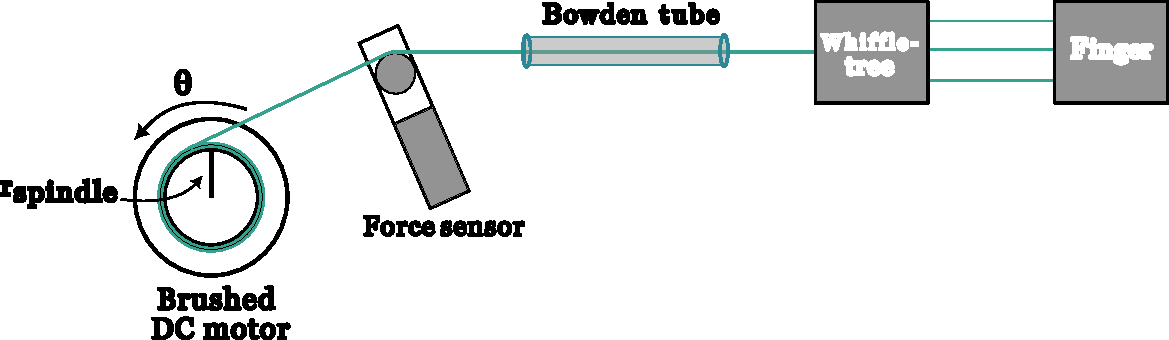
\includegraphics[width=1.0\textwidth]{../Figures/Introduction/setup.pdf}
    \caption{Simplified diagram of one motor actuating a finger.}
    \label{fig:introduction_setup}
\end{figure}

\begin{figure}[htbp]
    \centering
    \adjincludegraphics[trim={\dimexpr(\width-\height)/2\relax} 0 {\dimexpr(\width-\height)/2\relax} 0, clip, width=1.0\textwidth]{../Figures/Introduction/system.jpeg}
    \caption{Image of the system without the cable, bowden tube, whiffle tree or glove. Image taken by Devon Rohlf.}
    \label{fig:introduction_hardware}
\end{figure}

\section{Outline of thesis}

The thesis is structured as follows: \cref{ch:theory} provides the theoretical background necessary for understanding the subsequent chapters, including anatomy, modelling, and control theory. \cref{ch:modelling} details the modelling of the finger dynamics using the Euler-Lagrange equations, and the dynamics of the brushed DC motors, as well as estimates of the model parameters. \cref{ch:controller_design} presents the design, analysis and simulation-based validation of a current controller, torque and force controller, and an adaptive position controller. \cref{ch:discussion} discusses the results and findings of the thesis, and provides an outlook on future work, and finally, \cref{ch:conclusion} concludes the thesis.

\section{AI declarations}
LLMs have been used to assist in development of this thesis. Claude Code and ChatGPT have been used for several purposes, including assisting in coding, debugging, and proofreading this thesis. However, the text, methods developed, and figures in this thesis are all human-made. All contributions by an LLM have been reviewed and approved line by line.

